\section{Results and Discussion} \label{sec:results}

% @RCK - writing group
% Structure your R&D section to say, for each hypothesis 1. What you're showing. 2. Here's the evidence.
% Combine these figures to support your conclusions.
%
% Think about making two-part figures, one with the time-series, and then a partner panel that has the final dominant comparisons (violin or box plots).
%
% Visually distinguish your figures so that the reader, at a glance, can tell what they're looking at. Consider color-coding the backgrounds, or having distinct plot types for different kinds of conclusions.
%
% If you MUST show a pile of time series, consider combining them into sets of panels. Say one big figure with all your timeseries, but quadrants showing each one as part A, B, C, etc.
%
% Typesetting point: italicize or bold or underline key points or terms, particularly treatment names

\subsection{Does gene duplication facilitate adaptive evolution?}

In a first set of experiments, we set out to test the influence of gene duplication on adaptive evolution in our study system.
In the context of our experiments, which tracked populations of Avida digital organisms competing for limited virtual resources, adaptive evolution corresponded to performance of tasks from the Logic-9 set.

Figure \ref{fig:results_panels} compares task count trajectories over evolutionary time between treatments, as well as task count distributions among final dominant lineages.
Under the slip-duplicate treatment, significantly higher task counts  evolved compared to the baseline treatment (two-tailed Mann-Whitney U tests, W = 562.5, Bonferroni-adjusted $p << 0.0001$).

This result aligns with existing findings across a broad variety of biological taxa and digital models that slip-duplication of genetic material can facilitate evolution of adaptive traits \citep{Koza:1995fr,Zhang:2003fw,Teichmann:2004cz}.
Indeed, in earlier-reported experiments, we additionally found that facilitation of adaptive evolution by gene duplications generalized to changing environments, where the set of rewarded tasks fluctuated across generations \citep{lalejini2017gene}.

% AML: Still not really sure how we want to present the results panels. Thoughts?
% MJW: The lower figure in each panel (which is an odd formatting choice: this is really a 6 panel figure you're treating as 3) does not need to be anywhere near the width it is.  The point of those time graphs, as far as I can tell, is to show that the end point is not inherently weird compared to the rest of the trajectory.  How about trying putting the two graphs of each panel side by side, possibly even by having the violin plot panels take up 2/3 of the horizontal real estate and/or maybe replacing the categorical x axis labels with 1, 2, 3 etc and explaining them in the caption?

\begin{figure}[!h]
  \centering
  \begin{adjustbox}{scale=0.8}
    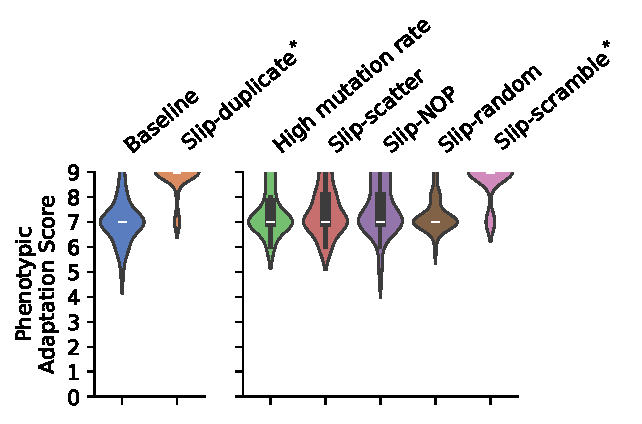
\includegraphics[
        height=4in,
        trim={0.2cm -1.5cm 0.2cm 0},
        clip
      ]{binder/binder/teeplots/col=split+env=static+hue=treatment+inner=box+kind=violin+palette=muted+viz=catplot+x=treatment+y=tasks-present+ext=.pdf}%
    \hspace*{-2.0cm}%
    \raisebox{0.125in}{%
      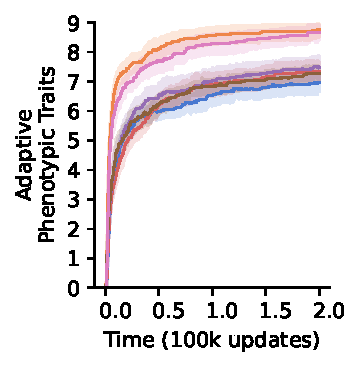
\includegraphics[
          height=2.7in,
          trim={1.36cm -0.64cm 0 0},
          clip
        ]{binder/binder/teeplots/env=static+errorbar=ci+hue=treatment+kind=line+palette=muted+viz=relplot+x=time-100k+y=tasks-present+ext=.pdf}}%
  \end{adjustbox}

  \vspace{-7ex}

  \begin{subfigure}{0.3\textwidth}
    \caption{\small slip-duplication}
    \label{fig:results_panels:slip_duplication}
  \end{subfigure}%
  \begin{subfigure}{0.35\textwidth}
    \caption{\small ablation treatments}
    \label{fig:results_panels:ablation}
  \end{subfigure}%
  \begin{subfigure}{0.22\textwidth}
    \caption{\small lineage history}
    \label{fig:results_panels:time_series}
  \end{subfigure}

  \vspace{1ex}

  \caption{\textbf{Treatments preserving slip-duplicated content facilitate adaptive evolution.}
    \small Violin plots show number of adaptive traits evolved in final dominant genotypes.
    Time series (\ref{fig:results_panels:time_series} right) shows progression of adaptive phenotypic trait counts along lineages of final dominant genotypes; color-coding corresponds to violin plots.
    Asterisk (*) markers indicate treatments with significantly more adaptive phenotypic traits compared to baseline, comparison across both \ref{fig:results_panels:slip_duplication} and \ref{fig:results_panels:ablation} panels.
    Simulation time unit is “updates,” corresponding to evaluation of ~30 genome sites per organism.}
  \label{fig:results_panels}
\end{figure}


\subsection{What aspects of gene duplication facilitate adaptation?}

Having observed that slip-duplicate mutations accelerate evolutionary acquisition of Logic-9 tasks in our model, we next sought to identify in greater detail which aspects of the slip duplication process, in particular, contribute to facilitating adaptation.
For this purpose, we extended our experiment to additionally include five variants of the slip-duplication operator, each disabling or replacing a particular functional aspect of slip duplication.
(Figure \ref{fig:slip_mut_variants} overviews variants tested.)

As shown in Figure \ref{fig:results_panels}, we detected significant increases in adaptive evolution against baseline only for the original slip-duplicate treatment and the follow-up slip-scramble treatment --- which ablated only sequence order within duplicated regions.
Task counts under all other experimental treatments were statistically indistinguishable, or slower-adapting, compared with the baseline treatment.

Given that the slip-scramble treatment maintains the content of duplicated instruction sequences (albeit, in an unordered fashion), these findings highlight an integral role for amplification of existing genetic information, in particular, with regard to how gene dulication promotes adaptive evolution in the study system.
In contrast to the slip-scramble and full slip-duplicate operators, other tested slip mutation variants do not duplicate information about instruction sequences already present in the genome.

Given the efficacy of the slip-scramble treatment in facilitating adaptation, we became curious as to the role of sequence order within duplicated regions.
To investigate this point, we additionally tested differences in task counts between the slip-scramble and slip-duplicate treatments.
To prevent issues with multiple comparison, we dispatced 100 new trials under both treatments for this test.

Indeed, this additional experiment confirmed that the slip-duplicate treatment did in fact yield higher task counts compared to the slip-scramble treatment (two-tailed Mann-Whitney U tests, W = 4305, 4028.5, 3621.5 respectively, Bonferroni-adjusted $p =$ 0.0109).
Thus, in our study system, it appears that the content and structure of duplicated genetic code contribute in promoting evolvability.
This finding further underscores that, in specific, the injection of existing sequence information is key to the role of gene duplication in evolution.

As above, earlier-reported experiments found that benefit to adaptive evolution from maintaining sequence order within duplicated regions generalized to changing environments where task rewards shifted with evolutionary time \citep{lalejini2017gene}.


\subsection{Discerning the Mechanism of Slip Duplication in Facilitating Adaptive Evolution}

Thus far, we have established that the locality and content of slip-duplicated genetic material both contribute substantially to its effectiveness in facilitating adaptive evolution.
We next sought to understand \textit{how} these mechanisms drive faster adaptive evolution.
In these investigations, we aimed to (1) identify how the effectiveness of gene duplication relates to trait complexity, (2) test for signatures of evolutionary potentiation by gene duplications along lineage histories, and (3) examine how slip duplication influences genetic architecture with respect to brittleness and vestigial genetic material.

\subsubsection{Slip duplication facilitates the evolution of complex traits.}

Within the logic-9 task system in Avida, available tasks vary substantially in their computational difficulty.
In fact, explicit hierarchical composition exists mong task definitions.
``Easier'' tasks like AND and NAND form building blocks for ``more difficult'' tasks like XOR and EQU.
Previous studies have used this property to explore the evolution of complex traits \citep{lenski2003evolution}.
We categorize the complexity of the Logic-9 tasks used in this work by the minimal number of NAND building blocks\footnote{
In computer architecture theory, NAND is commonly established as the fundamental building block operation since all other logical operations can be derived from compositions of NAND gates \citep{mano1997logic}.
} required to perform them:
\begin{enumerate}
\item NOT and NAND: one NAND component,
\item AND and ORNOT: two NAND components,
\item OR and ANDNOT: three NAND components,
\item NOR and XOR: four NAND components, and
\item EQU: five NAND components.
\end{enumerate}
We leveraged this natural hierarchy to test how gene duplication facilitates evolution across a spectrum of task complexities by studying the rate at which tasks with different NAND ``component counts'' evolved.

As explored earlier, one intrinsic consequence of gene duplication is increased genome length.
To account for this effect, we considered an additional control in our experiments: the long-genome baseline treatment, in which organisms employed fixed-length 1,000-site genomes.

\begin{figure*}
    \centering
    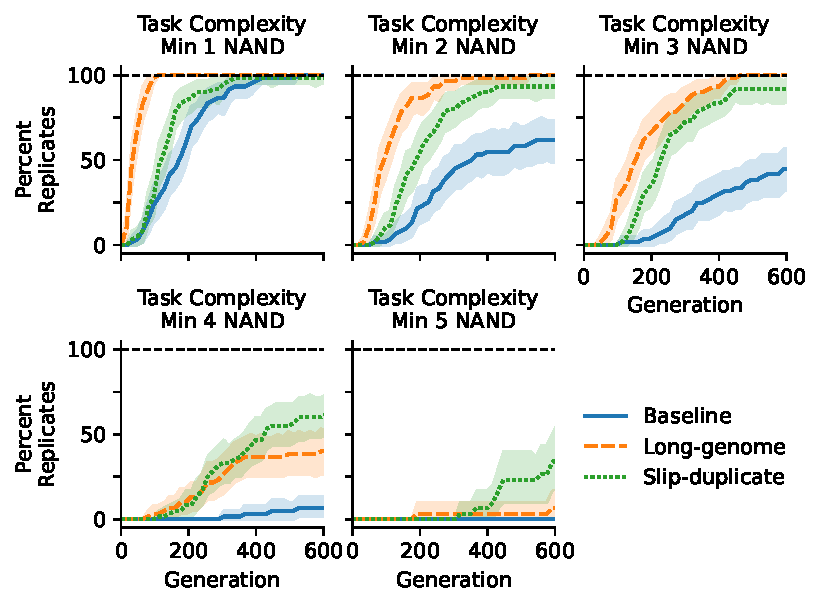
\includegraphics[width=\linewidth]{binder/binder/teeplots/adaptive-evolution-rate.ipynb/col=task-complexity+errorbar=ci+hue=treatment+kind=line+mutation=per site+post=plt-xlim-0-600+style=treatment+viz=relplot+x=generation+y=has-task+ext=.pdf}
    \caption{
        \textbf{Gene duplication boosts adaptive evolution of complex phenotypic traits.}
        \footnotesize
        Plots show fraction of replicates exhibiting available phenotypic traits, by generation from founding ancestor.
        Panels facet by trait complexity, measured by the minimum number of NAND operations required to complete the task.
        Simple tasks (top left) require only one NAND operation.
        More complex tasks (bottom right) require up to five NAND operations as shown in Figure \ref{fig:slip_mut_variants}.
        Slip-duplication treatment facilitates significantly faster adaptive evolution than long-genome treatment for the more complex tasks that require 4 or 5 subcomponents.
        Error bands give 95\% CI, bootstrapped over 30 replicates per treatment.
    }
    \label{fig:adaptive-evolution-rate}
\end{figure*}


First, we compared the adaptive boost from slip duplication against that from simply having longer genomes.
Figure \ref{fig:adaptive-evolution-rate} shows rates of task acquisition with and without slip duplication, including this long-genome control.

The long-genome control matched or exceeded the performance of slip-duplication in evolving simple traits with 3 or fewer components.
% https://github.com/chaynes2019/AvidaGeneDupe/blob/538ede79c7301f10718ca96c8dd38782b6882632/binder/adaptive-evolution-rate.ipynb
However, slip duplication evolved more complex 4- and 5-component traits in a significantly higher fraction of replicates compared to the long-genome control (Fisher's exact tests; 36/60 vs. 24/60, $p<0.05$ [4 components]; 10/30 vs. 2/30, $p<0.03$ [5 components]; Figure \ref{fig:adaptive-evolution-rate}).
As such, these findings lend support to hypotheses around gene duplication as a catalyst for the evolution of complex traits \citep{ohno1970evolution}.

\subsubsection{Slip-duplicated genome regions potentiate evolution of novel complex traits.}

% https://github.com/chaynes2019/AvidaGeneDupe/blob/4c7fa27229094adcb5bdb0b1aec541d0014b0fed/binder/hard-task-gain.ipynb
%             H-statistic       p-value
% Components
% 1              1.011820  3.144672e-01
% 2             22.787798  1.809107e-06
% 3             33.846753  5.962854e-09
% 4             15.359894  8.885441e-05
% 5              9.097744  2.559249e-03
%    Components  Prev Slip Insertion Cumulative Count      mean       std
% 0           1                                 False  0.932088  0.455109
% 1           1                                  True  1.002025  1.164197
% 2           2                                 False  0.588566  0.618479
% 3           2                                  True  1.579974  1.191681
% 4           3                                 False  0.491481  0.700256
% 5           3                                  True  1.516115  0.911430
% 6           4                                 False  0.703793  0.980105
% 7           4                                  True  1.229158  0.654042
% 8           5                                 False  0.583674  0.927917
% 9           5                                  True  1.249985  0.531423
%    Components  Prev Slip Insertion Cumulative Count  size
% 0           1                                 False    60
% 1           1                                  True    48
% 2           2                                 False    60
% 3           2                                  True    56
% 4           3                                 False    60
% 5           3                                  True    59
% 6           4                                 False    52
% 7           4                                  True    52
% 8           5                                 False    20
% 9           5                                  True    20

\begin{figure}
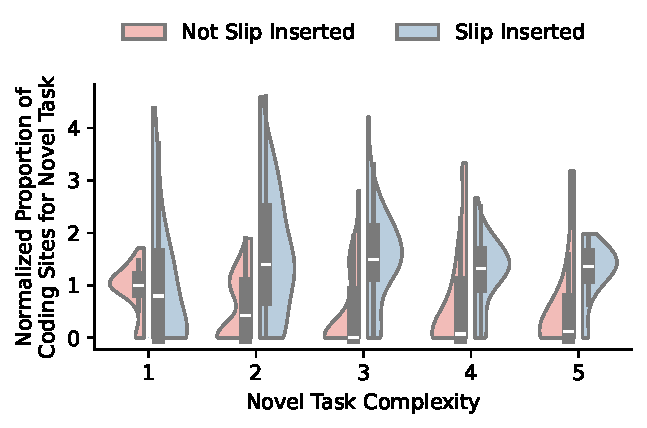
\includegraphics[
width=\linewidth
]{binder/binder/teeplots/density-norm=width+hue=prev-slip-insertion-cumulative-count+kind=violin+viz=catplot+x=components+y=is-task-coding-site+ext=.pdf}
\caption{%
  \textbf{Slip-duplicated sites are overrepresented among \textit{de novo} coding sites for complex traits.}
  \footnotesize
  Distributions compare frequencies of previously slip-duplicated and non-slip-duplicated sites among  \textit{de novo} task coding sites, normalized to neutral expectation.
  Values greater than 1 indicate that sites are overrepresented among the coding sites of novel traits compared to their background frequency.
  Differences between slip-duplicated and non slip-duplicated sites are significant for tasks requiring 2 or more NAND components (Mann-Whitney test; $p < 0.01$).
} \label{fig:potentiation}
\end{figure}


Thus far, we have established that slip duplication facilitates evolution of novel complex traits, we next sought to identify the processes through which slip duplication promotes adaptive evolution.
To this end, we tested whether slip duplication potentiates the evolution of adaptive traits at duplicated genome sites.
For each occurrence of a new trait arising in our experiments, we assessed the fraction of new task coding sites originating in regions of the genome that had previously been slip duplicated.
Figure \ref{fig:potentiation} compares these ratios of involvement in coding for new tasks between previously slip-duplicated and non-slip-duplicated sites.
For the simplest tasks, requiring only one NAND component, we found no significant difference in the likelihood of duplicated sites participating in coding regions for new tasks.
However, we found significant associations for traits with two or more NAND components (Mann-Whitney tests; all $p < 0.01$; $n=48,56,59,52,20$ observations).
Effect sizes of potentiation on likelihood to code for novel traits were $1.5\times$, $1.5\times$, $1.2\times$, and $1.2\times$ respectively for 2, 3, 4, and 5 task components.
Smaller effect sizes at 4- and 5-component tasks may be due to a larger portion of the genome becoming comprised of slip-duplicated sites (Supplementary Figure \ref{fig:potentiation-supp}), thus limiting the ceiling on deviation from expected.

One possible confounding factor in this result is reduced evolutionary rates at genome sites involved in organsims' self-replication loop.
These sites are critical to viability, with lethal outcomes when knocked out.
We found that these critical sites were less likely to be involved in slip duplication and also less likely to be involved in coding for \textit{de novo} traits.
Hence, sensitivity at these sites could introduce a spurious correlation.
However, we found similar potentiation signatures from slip duplication after excluding such fitness-critical slites from analysis (Supplemental Figure \ref{fig:potentiation-supp}).

One alternative to the potentiation hypothesis is that gene duplication directly facilitates adaptation by supplying mutational steps biased to discover beneficial outcomes \citep{kondrashov2012gene}.
Where regularities exist in the genotype-phenotype-fitness map, duplicated variants of existing genetic information may be more likely to encode meaningful traits.
In the fitness landscape analogy, this hypothesis would correspond to steps through fitness space that are larger but less risky.

In line with this possibility, we observed that a substantial fraction of gain-of-function steps on lineages directly coincided with slip duplications (TODO quantify).
However, in these cases, sites that gained a new trait directly due to slip mutation were nonetheless more likely than chance to have been involved in earlier slip duplications (Supplemental Figure \ref{fig:potentiation-supp}).
Thus, the adaptive characteristics of slip duplication seem likely to result from a combination of potentiation and direct facilitation.

\subsubsection{Gene duplication increases accumulation of vestigial coding material rather than decreasing genetic brittleness.}

\begin{figure}
    \centering
    \begin{subfigure}{\linewidth}
    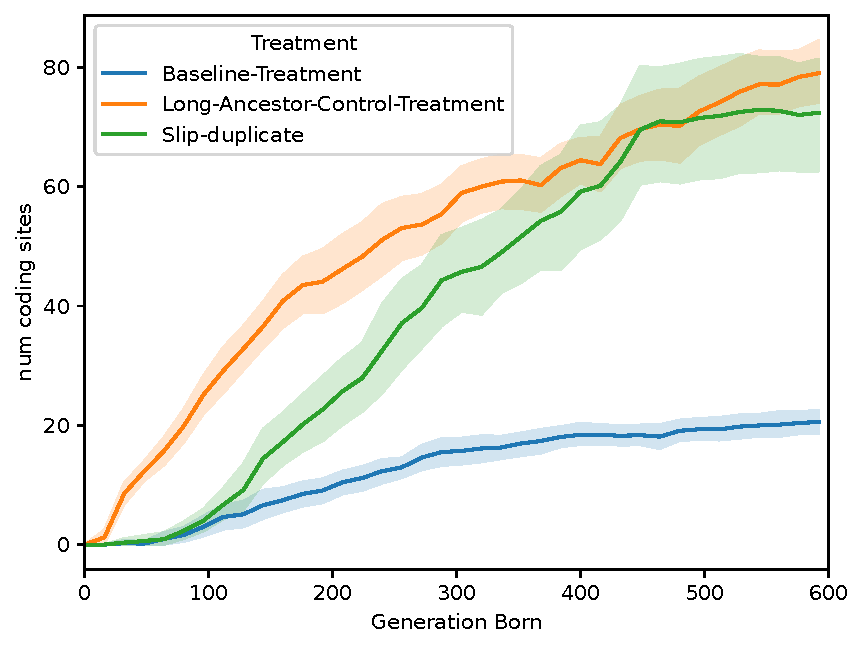
\includegraphics[width=\linewidth]{binder/binder/teeplots/hue=treatment+post=plt-xlim-0-600+viz=lineplot+x=generation-born+y=num-coding-sites+ext=.pdf}
    \caption{\footnotesize active coding sites}
    \label{fig:num-coding-sites:active}
    \end{subfigure}

    \begin{subfigure}{\linewidth}
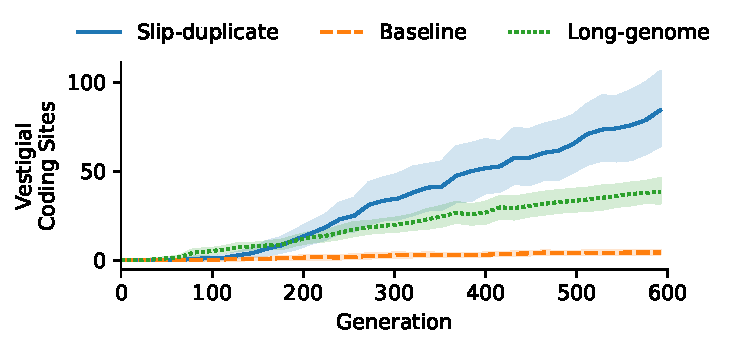
\includegraphics[width=\linewidth,clip, trim=0 0 0 0.8cm]{binder/binder/teeplots/hue=treatment+post=plt-xlim-0-600+viz=lineplot+x=generation-born+y=num-free-sites+ext=.pdf}
    \caption{\footnotesize vestigial coding sites}
    \label{fig:num-coding-sites:vestigial}
    \end{subfigure}
    \caption{
        \textbf{Gene duplication boosts accumulation of vestigial coding sites.}
        \footnotesize
        Generation-by-generation counts of coding sites over evolutionary history.
        Here, ``active'' coding sites refer to genome instructions determined through knockout to contribute to fitness with respect to self-copy viability or a rewarded phenotypic trait.
        As shown in panel \ref{fig:num-coding-sites:active}, gene duplication yields active coding site counts comparable to long-genome control.
        Vestigial coding site count, by contrast, reports the number of sites determined to have contributed to fitness in an ancestor, but are no longer active coding sites.
        As shown in panel \ref{fig:num-coding-sites:active}, vestigial coding site count under slip-duplication treatment outpace control treatments.
        Error bands give 95\% CI, bootstrapped over 30 replicates per treatment.
    }
    \label{fig:num-coding-sites}
\end{figure}


In a final set of analyses, we investigated broader relationships between gene duplication and genome architecture.

To assess effects on genome robustness, which we considered a definition in terms of brittleness;
that is, the number of genome sites ``critical'' to fitness, where a single-site knockout causes the loss of one or more adaptive phenotypic traits (i.e., tasks).
Single-site knockouts were used to identify critical sites via Avida's genome evaluator.\footnote{%
Although sufficiently representative for our purposes, limitations do exist in detecting Avida genome functionality through single-site knockouts; such an approach can underestimate aspects of genome sequence complexity involving small effects or redundancy \citep{moreno2024cryptic}.
}

We found that, rather than decreasing net brittleness, the slip duplication treatment accrued fitness-critical sites at a generation-on-generation rate comparable to the long-genome baseline treatment (Figure \ref{fig:num-coding-sites}).
However, slip duplications significantly increased the net amount of vestigial and active coding sites accrued in genomes (Figure \ref{fig:num-coding-sites}).
Thus, gene duplication increased supply of coding material in the genome available to neutral processes, even though overall robustness did not increase.
% https://github.com/chaynes2019/AvidaGeneDupe/blob/538ede79c7301f10718ca96c8dd38782b6882632/binder/indel-effect-nulldist.ipynb

In follow-up experiments, we tested the baseline effects of slip insertion mutations on brittleness without selection.
We found that slip insertions that were fitness-neutral tended to reduce net brittleness.
On average, these insertion mutations decreased coding site count by 6.8 sites.
This effect was strongest in genomes with high complexity; for instance, neutral insertion mutations decrease coding site count by 9.2 and 8.3 sites on average in genomes that encode 4- and 5-component complexity tasks, respectively.
Supplementary Figure \ref{fig:nulldist} overviews these results.
% One possible explanation is that selective pressures are driving the two treatments to reach a similar number of critical sites, but slip duplication can duplicate and copy genome content in a manner that increases the copy count of previously coding sites relative to the number of critical sites.



\subsection{Major Results}

We found local slip mutations of intact regions to be the most effective configuration of gene duplication in facilitating evolution on the logic-9 task set within the Avida platform.
In particular, we found that --- compared to control experiments with long genome sizes --- gene duplication uniquely promoted the evolution of complex adaptive traits.
We further found that the raw material created by slip duplication plays a potentiating role in the evolution of complex traits.
Specifically, we identified that slip-duplicated regions are significantly more likely to provide coding sites for new traits when they first appear.
Consistent expectations under neofunctionalization theory, however, we did not observe potentiation effects of slip duplication on the evolution of very simple traits that did not involve building block components.

Finally, we assessed the consequences of slip duplication on genome architecture.
One possible expectation is that gene duplication might accelerate growth in genetic brittleness by providing raw material for contingent complexity to arise, as drift effects wear away the redundancies introduced by duplication.
Contrary to this expectation, we found that the rate of genome complexity growth was similar to that observed in control experiments.
However, we observed a significant increase in the accumulation rate of net active and vestigial coding material in genomes under slip duplication.
To understand this phenomenon, we tested the immediate effects of slip duplication on genome brittleness.
We found that, on average, neutral slip duplications decrease, rather than increase, the number of critical coding sites in a genome.
These results align with our observed increase in vestigial coding material in genomes.
These brittleness-reducing effects appear to be counteracted by other factors, resulting in a similar overall trajectory of genome complexity between slip duplication treatments and controls.

\subsubsection{Outro/pitch.}
Strong theoretical interest exists in characterizing the role of gene duplication in facilitating neutral evolution and enabling adaptive evolution of new complexity through subfunctionalization and neofunctionalization.
Indeed, ample evidence from existing experiments \textit{in silico} and \textit{in vivo} has supported the role of gene duplication in facilitating the evolution of novelty, complexity, and adaptation.
Our study contributes to this conversation by highlighting in greater detail and specificity the consequences of gene duplication in a full-fledged digital model:
\begin{enumerate}
\item While increasing the amount of raw genetic material suffices to facilitate the evolution of simple traits, duplicating existing genome material excels in facilitating the evolution of complex traits;
\item Mechanistically, duplications significantly potentiate genome regions that go on to code for novel complex traits but --- consistent with neofunctionalization theory --- do not potentiate simple traits;
\item From a genetic architecture perspective, we do not find direct evidence of subfunctionalization in increasing genome brittleness under slip duplication; however, slip duplication accelerates the accumulation of net vestigial and active coding material in genomes.
\end{enumerate}

% \subsection{High mutation rate inhibits the evolution of regulation in changing environments}
% In addition to our results on why gene duplications promote evolvability, our experiments
% %demonstrate the potential for
% indicate that
% high mutation rates inhibit the evolution of regulation in changing environments. In both the simple and complex changing environments, organisms evolved in the high mutation rate treatment had significantly lower phenotypic match scores than organisms evolved in the baseline treatment, which can be seen in Figure \ref{fig:results_panels} (two-tailed Mann-Whitney U tests, W = 9958 and 9944, respectively, Bonferroni-adjusted $p$ values both $<< 0.0001$).
% A similar result was found in \citep{Lalejini:2016plasticity}. Although higher mutation rates increase genetic variation, most mutations have deleterious effects \citep{Schlichting:2002jl}. Thus, higher mutation rates may increase the difficulty of maintaining the genetic machinery necessary for complex regulation.

% If elevated mutation rates %can work to
% inhibit the evolution of regulation and all experimental treatments with slip mutation operators have an effectively higher mutation rate than the baseline treatment, why do we see this effect only in the high mutation rate treatment? The rates of insertions and deletions per instruction copied in the high mutation rate treatment were selected to, on average, result in approximately the same number of mutations per divide as in our treatments with slip mutations. Yet, only organisms evolved in the high mutation rate treatment had significantly lower phenotypic match scores than organisms evolved in the baseline treatment in the changing environments; all other experimental treatments were either significantly better or not significantly different than the baseline treatment.

% @amlalejini old text on mutation load explanation:
%Why is it that \textit{only} the high mutation rate treatment inhibited evolvability in the changing environments? One possibility is because slip mutations result in large mutational events that affect few offspring, whereas mutations in the high mutation rate treatment result in an increased number of smaller mutational events that are spread across many offspring. Thus, many offspring in the high mutation rate treatment are subject to the increased rate of deleterious mutations that results from an increase in the rates of copy insertions and copy deletions. This is in contrast to treatments with slip mutations where relatively fewer offspring are subjected to the increased rate of deleterious mutations because deleterious mutations are concentrated in a fewer offspring relative to the high mutation rate treatment.
%Further analysis is needed to confirm that this is, indeed, the case.
% @amlalejini new text on mutation load explanation:
%  - should I cite something for 'mutation load' (i.e. this concept exists, read about it here)?
% Why is it that \textit{only} the high mutation rate treatment inhibited evolvability in the changing environments?
% One possibility stems from the higher mutation load imposed on populations by the high mutation rate treatment.
% Slip mutations result in large mutational events that affect few offspring, whereas the elevated rate of copy mutations in the high mutation rate treatment results in an increased number of smaller mutational events spread across many offspring.
% Thus, many offspring in the high mutation rate treatment are subject to the increased rate of deleterious mutations that results from the higher rates of copy insertions and copy deletions. This is in contrast to treatments with slip mutations where relatively fewer offspring are subjected to large mutational events, which results in the concentration of deleterious mutations in fewer offspring relative to the high mutation rate treatment.
% Further analysis is needed to confirm that this is, indeed, the case.

% OLD figures
% \begin{figure}
    \centering
    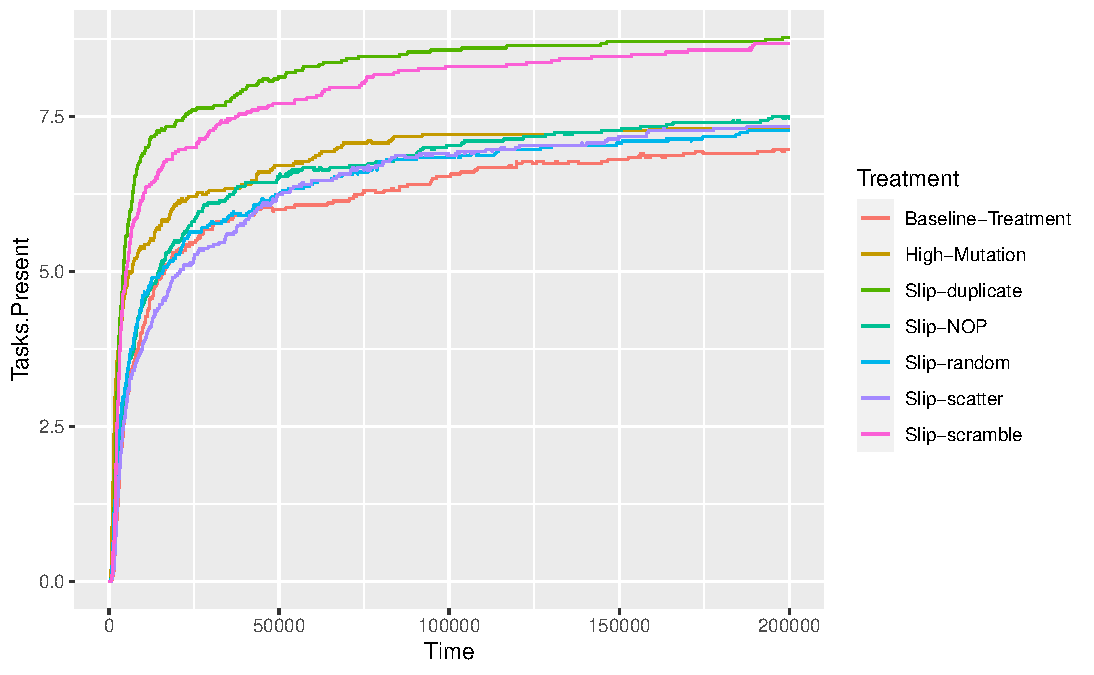
\includegraphics[width=\linewidth]{img/2022-3-29-PaperDuplication/TidiedData/FullReplicationTaskCountTimeCourse}
    \caption{TODO} \label{fig:FullReplicationTaskCountTimeCourse}
\end{figure}

% \begin{figure}
    \centering
    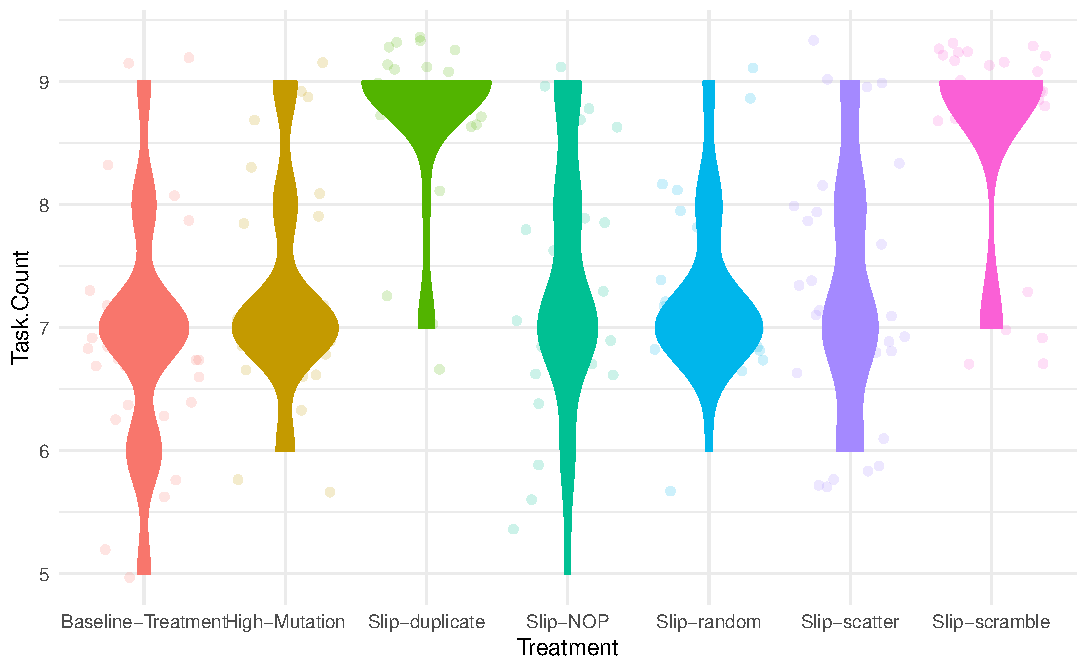
\includegraphics[width=\linewidth]{img/2022-3-29-PaperDuplication/TidiedData/FullReplicationFinalDominantTaskCountViolin}
    \caption{TODO} \label{fig:FullReplicationFinalDominantTaskCountViolin}
\end{figure}

% \begin{figure}
    \centering
    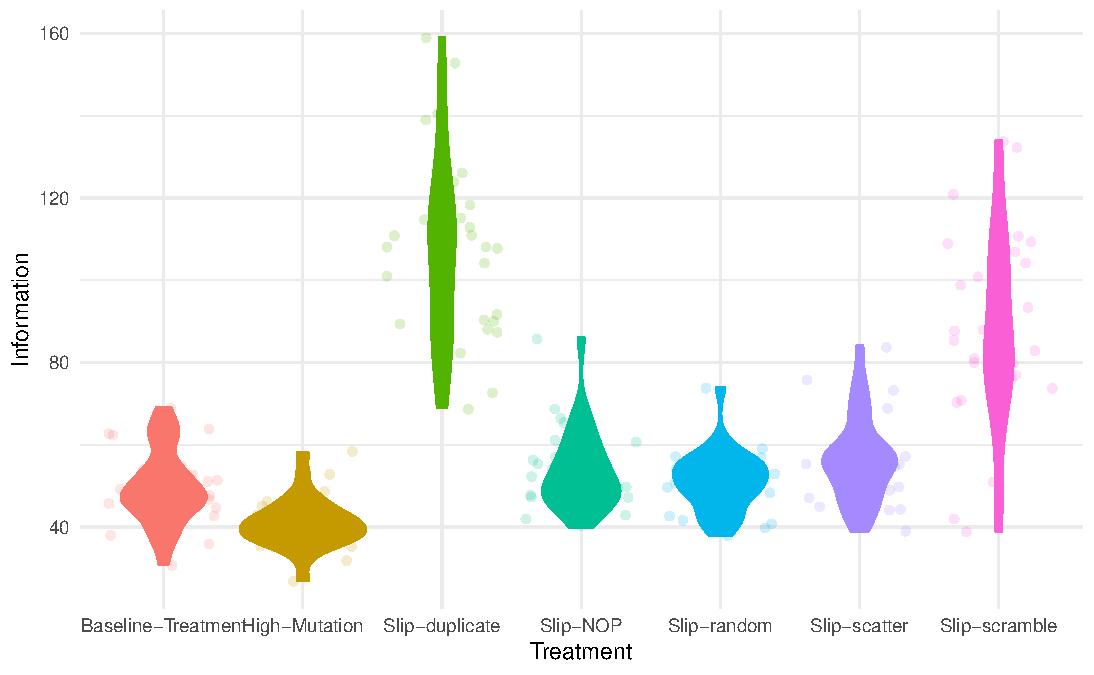
\includegraphics[width=\linewidth]{img/2022-3-29-PaperDuplication/TidiedData/LalejiniEtAlReplicationFinalDominantInfo}
    \caption{TODO} \label{fig:LalejiniEtAlReplicationFinalDominantInfo}
\end{figure}

% \begin{figure}
    \centering
    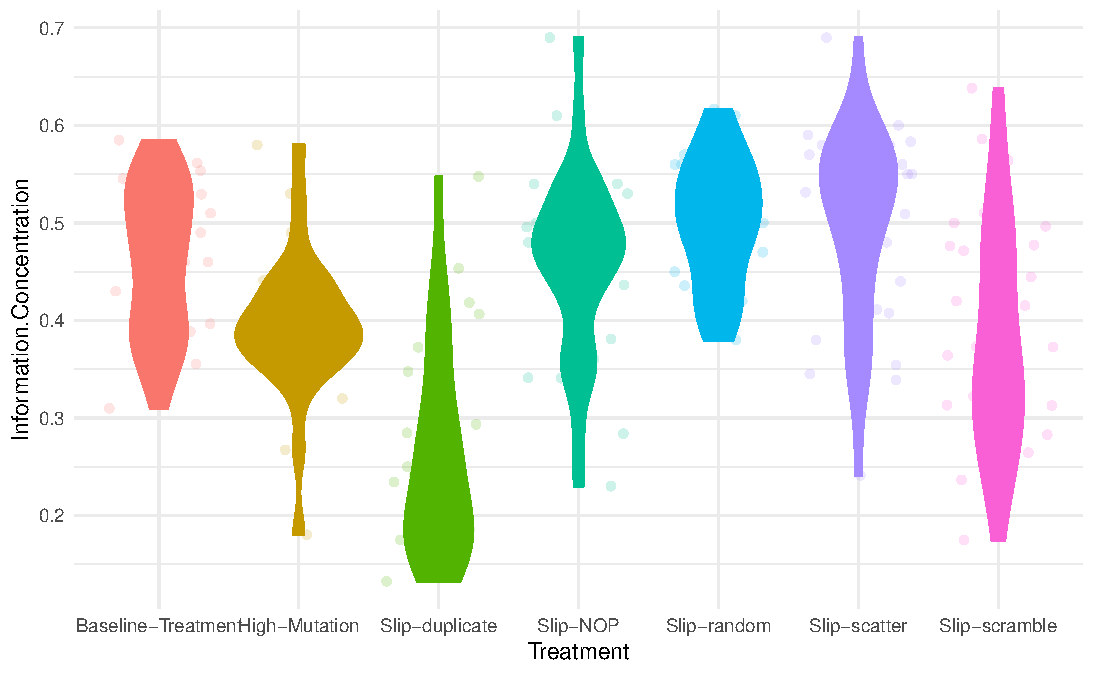
\includegraphics[width=\linewidth]{img/2022-3-29-PaperDuplication/TidiedData/LalejiniEtAlReplicationFinalDominantInfoConcentration}
    \caption{TODO} \label{fig:LalejiniEtAlReplicationFinalDominantInfoConcentration}
\end{figure}

% \begin{figure}
    \centering
    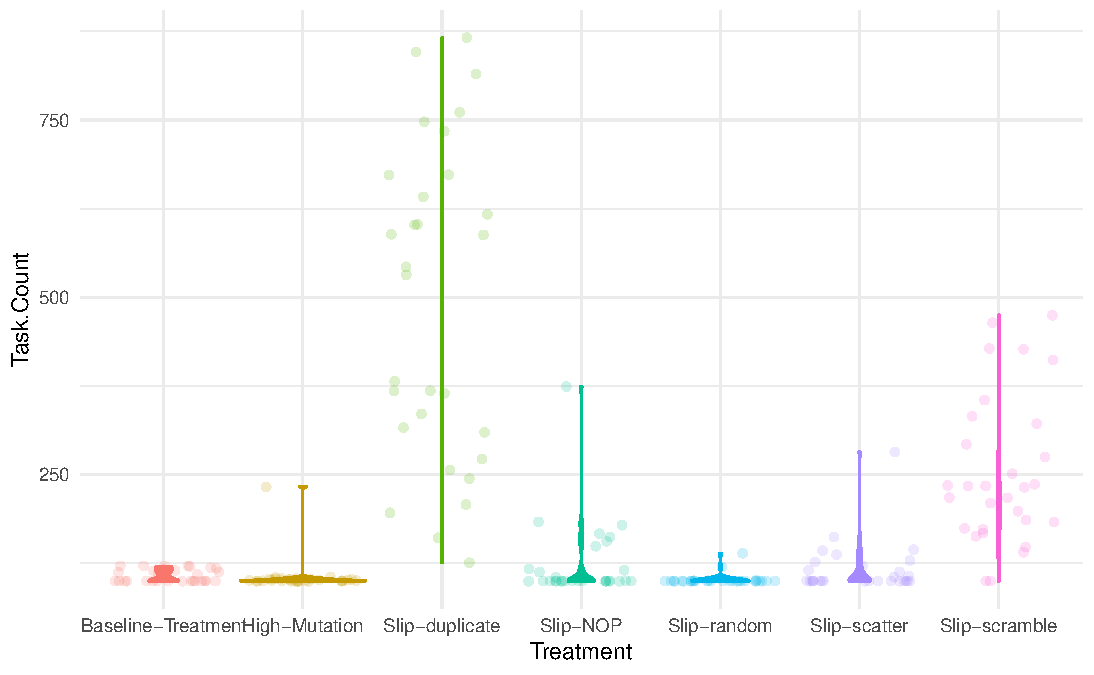
\includegraphics[width=\linewidth]{img/2022-3-29-PaperDuplication/TidiedData/LalejiniEtAlReplicationFinalDominantGenomeLengthsViolin}
    \caption{TODO} \label{fig:LalejiniEtAlReplicationFinalDominantGenomeLengthsViolin}
\end{figure}

% \begin{figure}
    \centering
    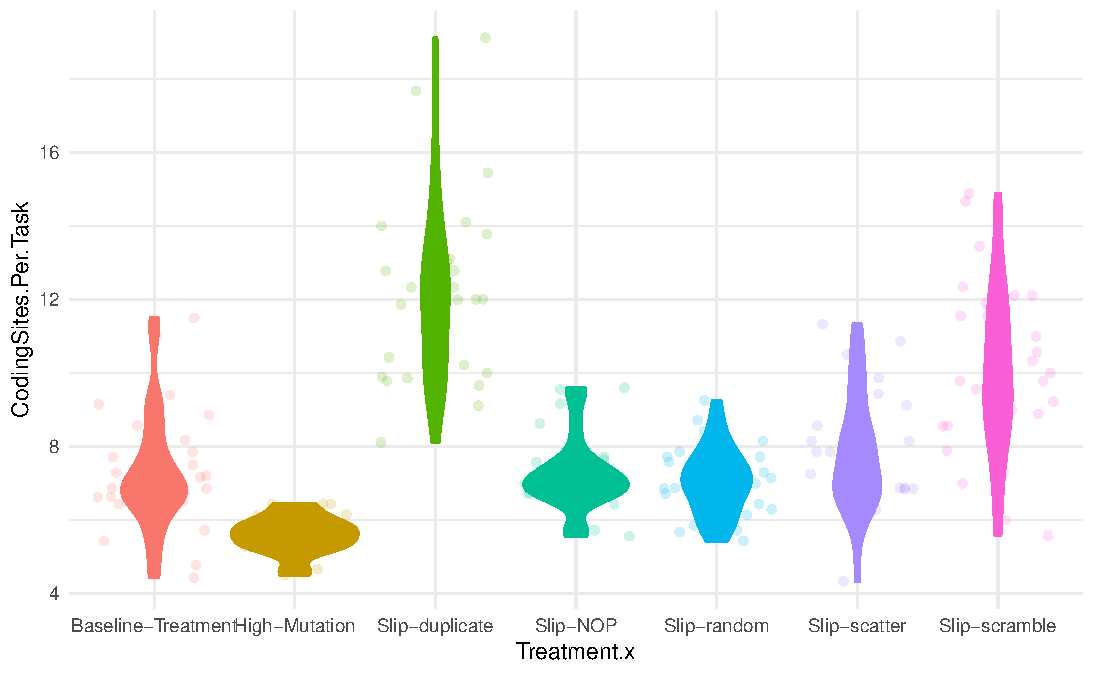
\includegraphics[width=\linewidth]{img/2022-3-29-PaperDuplication/TidiedData/LalejiniEtAlReplicationFinalDominantCodingSitesPerTask}
    \caption{TODO} \label{fig:LalejiniEtAlReplicationFinalDominantCodingSitesPerTask}
\end{figure}

% \begin{figure}
    \centering
    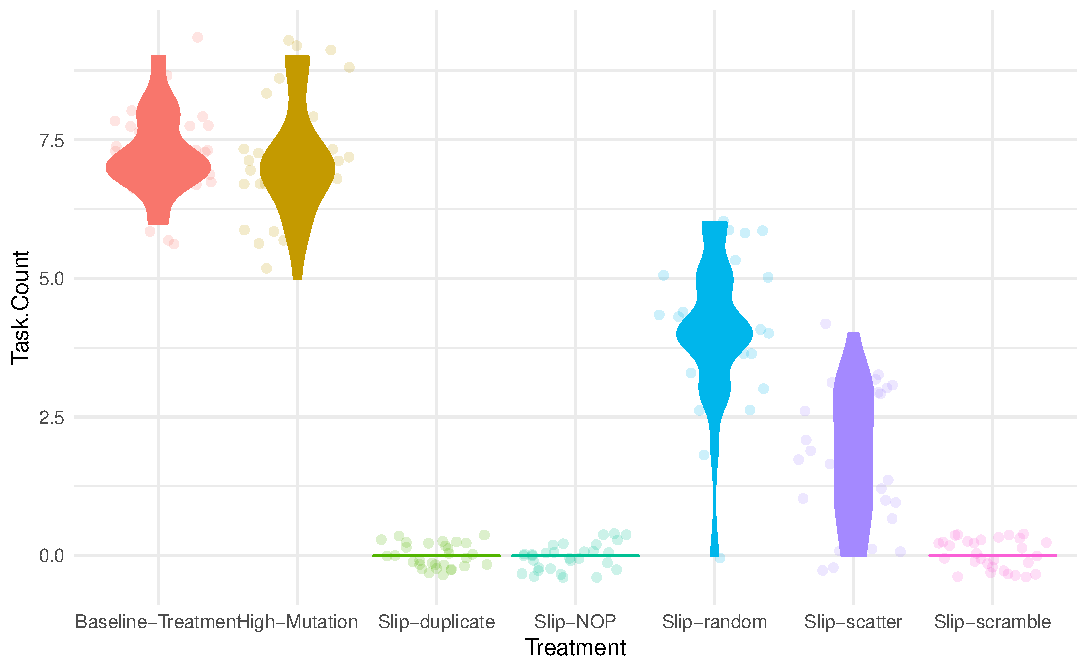
\includegraphics[width=\linewidth]{img/2022-3-29-PaperDuplication/TidiedData/ModifiedReplicationFinalDominantTaskCountViolin}
    \caption{TODO} \label{fig:ModifiedReplicationFinalDominantTaskCountViolin}
\end{figure}

% \begin{figure}
    \centering
    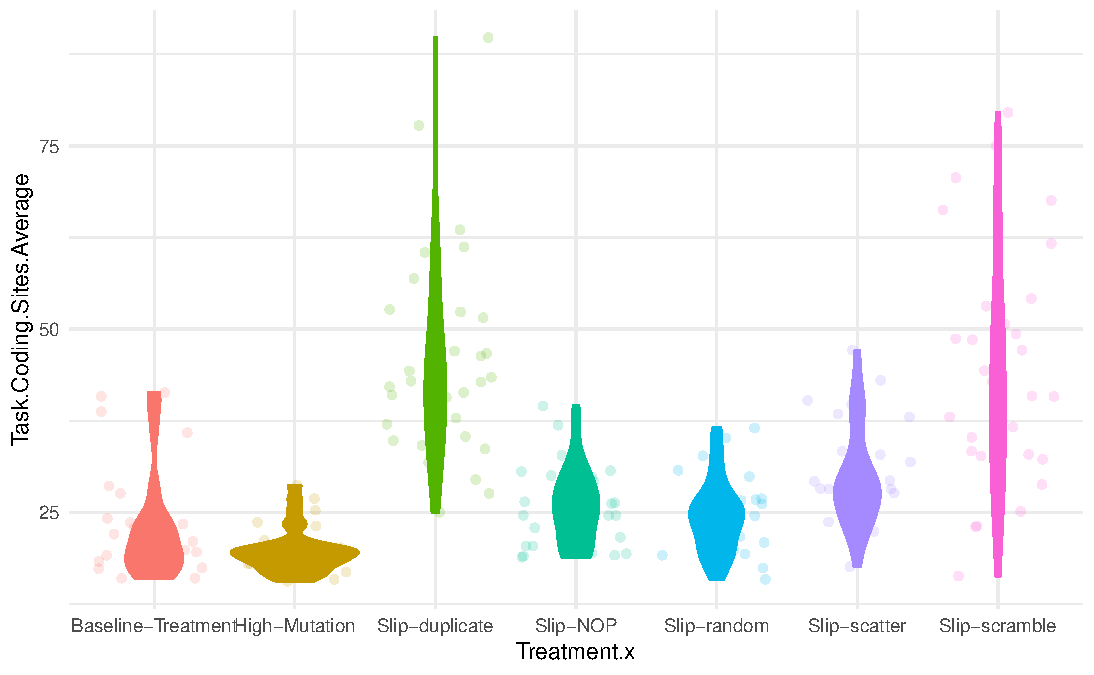
\includegraphics[width=\linewidth]{img/2022-3-29-PaperDuplication/TidiedData/LalejiniEtAlReplicationRealFinalDominantCodingSitesPerTask}
    \caption{TODO} \label{fig:LalejiniEtAlReplicationRealFinalDominantCodingSitesPerTask}
\end{figure}

% \begin{figure}
    \centering
    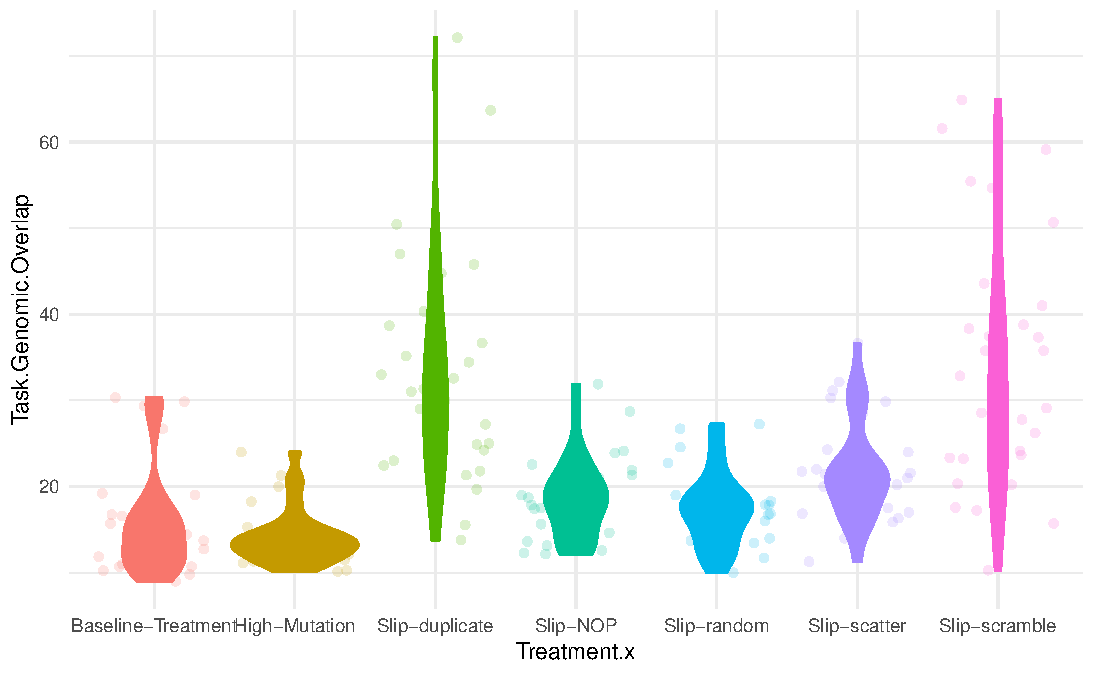
\includegraphics[width=\linewidth]{img/2022-3-29-PaperDuplication/TidiedData/LalejiniEtAlReplicationFinalDominantOverlap}
    \caption{TODO} \label{fig:LalejiniEtAlReplicationFinalDominantOverlap}
\end{figure}

